\chapter{Praktische Evaluation}

\section{Testumgebung}
Die folgenden Experimente wurden auf mithilfe einer AMD EPYC 7763 64-Core CPU mit 16 nutzbaren Hardwarethreads und 64GB Arbeitsspeicher durchgeführt. Das System
verwendet Ubuntu 24.04 als Betriebssystem und GCC in der Version 13.2.0 als Compiler. Die Ausführung der Algorithmen mit einer spezifischen Anzahl von Threads wurde
softwareseitig über OpenMP-Instruktionen realisiert. 

\section{Implementierung}

\subsection{Klassenstruktur}
\begin{figure}[h]
    \centering
    \caption{Klassenstruktur der Implementierung}
    \includegraphics[scale=0.4]{Images/uml.png} \label{uml}
\end{figure}

Die in \ref{uml} dargestellte Klassenstruktur illustriert die grundlegende Abstraktion, die für die Implementierung der Algorithmen verwendet wurde. Compressor und
Coder beschreiben jeweils ein Interface bzw. ein Template, welches durch ein konkretes Kompressionsverfahren und einer Kodierung spezialisiert werden kann. Jegliche
Spezialisierungen teilen sich jedoch eine gemeinsame Definition eines Faktors im LZ77-Schema.

\subsection{Code}
Die konkrete Implementierung erfolgte in der Programmiersprache C++ im C++20 - Standard und dem Build - System CMake in der Version 3.28. Die Parallelisierung wurde
über Präprozessor - Instruktionen von OpenMP realisiert.

\section{Messung}

\subsection{Eingabedaten}
Die folgenden Algorithmen wurden auf verschiedenen Dateien aus dem Pizza \& Chili-Corpus getestet. Die verwendeten Dateien decken verschiedene Kontexte und damit
Kompressionspotentiale ab.
\begin{figure}[h]
    \centering
    \caption{Auflistung der verwendeten Eingabedaten}
    \label{inputdata}
    \begin{tabular}{|c|c|c|c|c|}
        \hline
        \textbf{Datei} & \textbf{Größe} & \textbf{Alphabetgröße} & \textbf{Beschreibung} \\
        \hline
        \texttt{dna} & 200MB & 4 & DNA-Sequenzen \\
        \hline
        \texttt{english} & 200MB & 256 & Englische Texte \\
        \hline
        \texttt{proteins} & 200MB & 20 & Proteinsequenzen \\
        \hline
        \texttt{sources} & 200MB & 256 & Quellcode \\
        \hline
        \texttt{xml} & 200MB & 256 & XML-Dateien \\
        \hline
    \end{tabular}
\end{figure}
In der Tabelle \ref{inputdata} sind die verwendeten Dateien aufgelistet. Die Größe der Dateien wurde auf 100MB beschränkt, um einen angemessenen Rahmen für die 
Laufzeitmessung zu erhalten.

\subsection{Messgrößen}

\subsubsection{Laufzeit}
Die Laufzeit der Algorithmen wurde innerhalb der Ausführung gemessen. Dabei wird die Zeitmessung nach dem Laden der Eingabedatei gestartet und mit dem vollständigen
Auffüllen der Faktorfolge beendet. Damit wird das Einlesen der Eingabe und eine eventuelle Kodierung der Ausgabe nicht in die Laufzeitmessung einbezogen. Diese Strategie
hat ihren Hintergrund in der Tatsache, dass die konkrete Ausprägung des Eingabe- und Ausgabestroms keine Aussagekraft über die Qualität der Kompression hat.

\subsubsection{Speicher}
Der Speicherverbrauch der Algorithmen wurde auch intern mithilfe einer externen Bibliothek gemessen. Dabei wurden Speicherallokationen auf dem Heap überwacht und 
gemessen. Im Rahmen dieser Arbeit wurde die Spitze des allokierten Speichers im Zeitraum nach dem Einlesen der Eingabedatei und nach dem vollständigen Auffüllen der
Faktorfolge gemessen.

\subsubsection{Kompressionsrate CR*}
Die Kompressionsrate wird neben der Anzahl der Faktoren zum Großteil von der verwendeten Kodierung bestimmt. Wie bereits erwähnt, sind wir in der Wahl der Kodierung
nicht beschränkt, sodass die Aussagekraft bezüglich der Qualität der Kompression nicht eingeschränkt ist. Es ist jedoch zu beachten, dass Faktoren, die durch Approx. LZ77
erzeugt werden stets eine Zweierpotenz als Länge annehmen. Die binäre Repräsentation dieser Längen kann daher in Abhängigkeit von der gewählten Kodierung kompakt 
konstruiert werden. Um dieses Phänomen zu illustrieren gehen wir im Folgenden eine naive Kodierung vor, auf dessen Grundlage wir die Kompressionrate $CR*$ definieren.
\begin{equation}
    |K_{LZ77}(f)| = 1 + \begin{cases}
        2\log_2(n) & \text{falls } |f| > 1 \\
        9 & \text{sonst}
    \end{cases}
\end{equation}
Im Falle von LZ77 bestimmt ein Bit, ob es sich um eine Referenz oder ein einzelnes Zeichen handelt. Im Falle einer Referenz wird die Länge und die Position der Referenz
mithilfe von $\log_2(n)$ Bits kodiert. Im Falle eines einzelnen Zeichens wird die ASCII-Kodierung des Zeichens verwendet, die 8 Bits benötigt.
\begin{equation}
    |K_{Approx.LZ77}|= 1 + \begin{cases}
        \log_2(n)+\log_2(\log_2(n)) & \text{falls } |f| > 1 \\
        9 & \text{sonst}
    \end{cases}
\end{equation}
Im Falle von Approx. LZ77 kann die Länge mithilfe von $\log_2(\log_2(n))$ Bits kodiert werden, da die Länge anhand einer einzelnen Bitposition bestimmt wird.

\newpage
\subsection{Messwerte}

\begin{table}[ht]
    \centering
    \caption{Messgrößen der Algorithmen}
    \label{messwerte}
    \begin{tabular} { |c|c|c|c|c|c| }
        \hline
        \textbf{Eingabe} & \textbf{Algorithmus} & \textbf{Laufzeit[s]} & \textbf{Speicher[Byte]} & \textbf{FR} & \textbf{CR*} \\
        \hline
        & LZ77 & 15.40 & 20.00 & 9.98\% & 70.83\% \\
        proteins & Approx.LZ77 & 44.06 & 9.94 & 15.34\% & 63.95\% \\
        & Approx.LZ77Par & 6.99 & 10.21 & 15.34\% & 63.95\% \\
        \hline
        & LZ77 & 13.47 & 20.00 & 5.60\% & 38.75\% \\
        sources & Approx.LZ77 & 40.43 & 6.42 & 10.05\% & 40.14\% \\
        & Approx.LZ77Par & 6.49 & 5.90 & 10.05\% & 40.14\% \\
        \hline
        & LZ77 & 15.36 & 20.00 & 6.70\% & 47.24\% \\
        english & Approx.LZ77 & 51.00 & 7.06 & 10.42\% & 43.39\% \\
        & Approx.LZ77Par & 7.46 & 6.16 & 10.42\% & 43.39\% \\
        \hline
        & LZ77 & 14.89 & 20.00 & 6.66\% & 47.46\% \\
        dna & Approx.LZ77 & 30.10 & 8.38 & 10.71\% & 45.53\% \\
        & Approx.LZ77Par & 4.80 & 6.66 & 10.71\% & 45.53\% \\
        \hline
        & LZ77 & 13.02 & 20.00 & 3.42\% & 23.61\% \\
        xml & Approx.LZ77 & 29.38 & 3.46 & 6.62\% & 26.78\% \\
        & Approx.LZ77Par & 4.91 & 3.46 & 6.62\% & 26.78\% \\
        \hline
    \end{tabular}
\end{table}

\subsubsection{Laufzeiten}
\begin{figure}[ht]
    \centering
    \caption{Laufzeitmessung von LZ77, Approx.LZ77 und Approx.LZ77Par(16 Threads) auf verschiedenen Präfixen von proteins. Als Vergleichsmaß wurde 
    die lineare Regression der Kurven gestrichelt eingezeichnet.}
    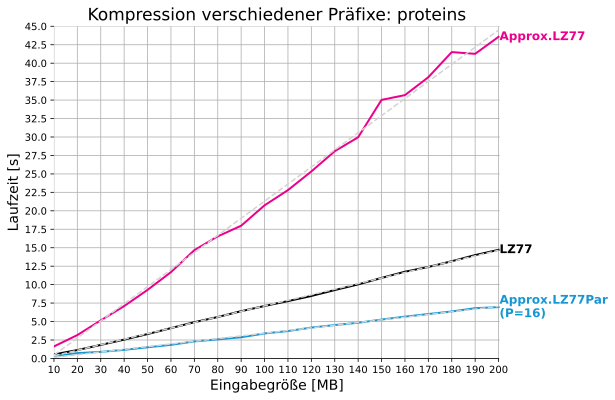
\includegraphics[scale=0.6]{Images/progressive_proteins.pdf}
\end{figure}
    
\begin{figure}[ht]
    \centering
    \caption{Laufzeitmessung von Approx.LZ77Par mit verschiedener Anzahl an Threads für proteins}
    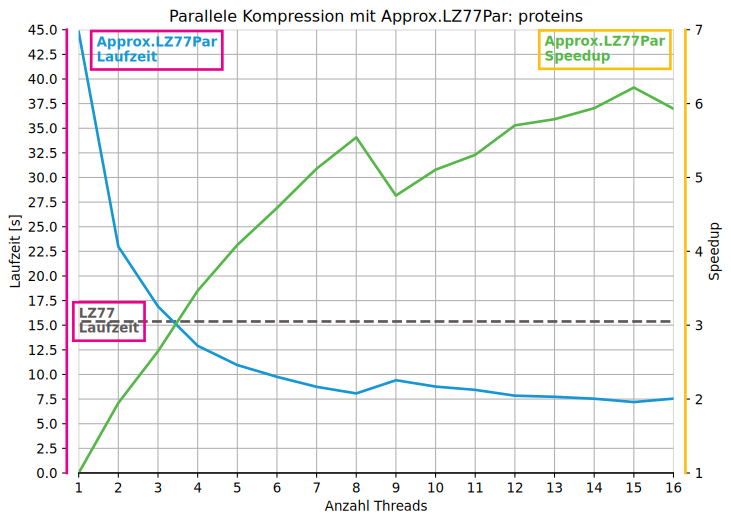
\includegraphics[scale=0.6]{Images/progressive_speedup_proteins.pdf}
\end{figure}

\subsubsection{Speicherverbrauch}
\begin{figure}[ht]
    \centering
    \caption{Speicherverbrauch von LZ77, Approx.LZ77 und Approx.LZ77Par(16 Threads) auf verschiedenen Präfixen von proteins. Aufgezeichnet wurde das Verhältnis
    von allokiertem Speicher zur Eingabegröße.}
    \includegraphics[scale=0.6]{Images/progressive_mem.pdf}
\end{figure}
\subsubsection{FR und CR*}

\section{Auswertung}
\subsection{LZ77}
\subsection{Approx. LZ77}
\subsection{Approx. LZ77Par}